\documentclass[12pt]{article}

\usepackage{amsmath}
\usepackage{graphicx}

\title{Generating Graphs With Specific Motif Counts}

\begin{document}
\maketitle

\section{Introduction}

Many real-world systems can be modeled by graphs, from power grids to arXiv citations to friendships on Facebook.  Early models attempted to model all systems with the same type of graph.  For example, the Erdos-Renyi random graph models all networks with $n$ participants and $m$ connections with a graph of $n$ nodes and $m$ randomly placed edges.  The Watts-Strogatz model models all networks by connecting nodes to their nearest neighbors, then filling the rest of the graph with randomly placed edges.

More sophisticated models account for differences in degree distribution and clustering coefficient.  The preferential-attachment model generates a graph with power-law degree distribution and allows the modeler to choose the exponent in the power law.  The configuration model takes as input an exact sequence of degrees and creates a random graph with that degree sequence.  Newman's "triangle-edge" model generalizes this to create a random graph with specific degree sequence and clustering coefficient.

In our model we create a random graph with specific degree sequence and motif counts.  A motif is a small subgraph (with fewer than five vertices), so we would create a graph with specific numbers of cycles, 4-cliques, etc.  While this problem is NP-hard [proved by Sen Wu, my CS224W project partner] and may not have exact solutions, we use hill-climbing to find an approximate solution that produces good results in practice.

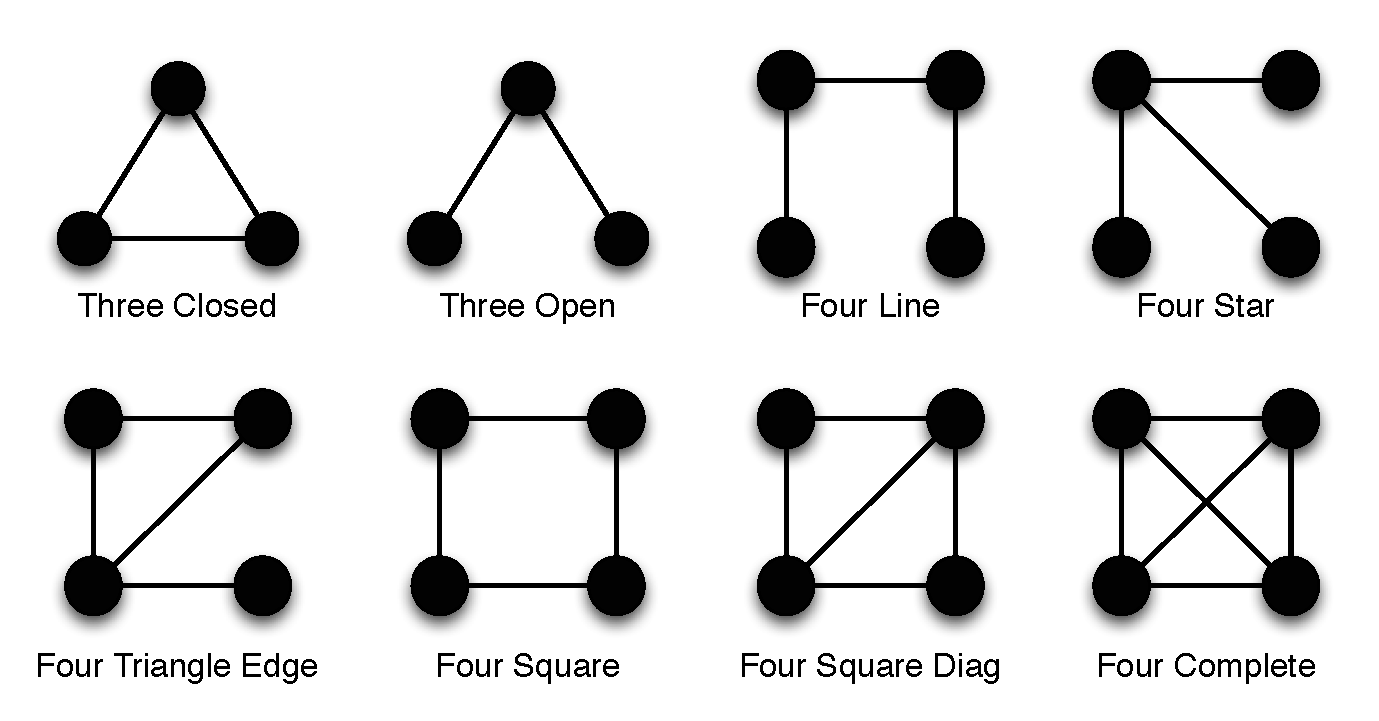
\includegraphics[scale=0.50]{motifs.eps}\\

Figure 1: Motifs we are considering.  [Credit: Sen Wu]

\section{Methods}
\subsection{Hill climbing}
Hill-climbing is a standard technique for finding good solutions to optimization problems.  Start with a solution that is not particularly good.  At each step, perturb the solution randomly.  If the new answer is better, keep it; if not, keep the old solution.  Repeat this until the algorithm converges to a good solution.

Hill-climbing does not guarantee an optimal solution, since it tends to get stuck at local maxima.  Yet in practice the solutions it finds are "pretty good," especially after running it several times and picking the best solution.

In our case we minimize the error between the desired motif counts and our solution's motif counts: [change denominator of error function?] $$\mbox{Average relative error} = \frac{1}{\ell} \sum_{i = 1}^{\ell} \frac{|counts_i - \widehat{counts}_i| + 1}{|counts_i| + 1}$$ where $\ell$ is the number of different motif types.

We use the configuration model to generate a random graph with the required degree sequence.  Then at each step we choose two edges (at random) and swap their endpoints.  (We chose this transformation step since it preserves the degree sequence of the graph.)  We count the motifs and compare the error with the new counts to the error with the old counts.  If the new counts give a smaller error, we keep the new graph; otherwise, we discard it.

\subsection{Optimizations}
As written, this solution is very slow.  Counting motifs is $O(|V|^4)$ and takes unacceptably long in practice.  To get good results in practice, we need at least as many rewiring steps as the number of edges in the graph [check this], so ideally each rewiring step should take less than a second.

We can speed this up by counting motifs incrementally.  Instead of considering the whole graph on every step, we only look at the part of the graph whose motifs would be affected by the edge changes.  Since we are only looking at motifs with fewer than $5$ nodes, we can only consider the nodes that are one or two hops away from the nodes whose edges are being rewired.  Then we can count how many motifs are being created or destroyed in the induced subgraph on those nodes, and add those to the total motif counts.  Once we have the induced subgraph, we count the motifs by taking all possible sets of four vertices, and seeing which motif they form, if any.

(Note that we break the rewiring step into four steps, two edge deletions and two edge creations.  This way we only measure the effect of one edge creation/deletion step at a time.)

This is still fairly slow, so we apply one final optimization.  We notice that for a 4-motif to be affected by the edge changes, vertices $1$ and $2$ of the motif must be endpoints of the edge.  Vertex $3$ must be an immediate neighbor of an endpoint, and vertex $4$ is either an immediate neighbor or a second-degree neighbor.  Ordinarily, we would have to loop through the immediate neighbors to find all possibilities for vertex $3$, and perform an inner loop through the second degree neighbors to find all possibilities for vertex $4$.  But if vertex $4$ was always an immediate neighbor, we could loop through the immediate neighbors both times, which would speed up the algorithm considerably.

Vertex $4$ is not always an immediate neighbor.  However, in the cases where it's not an immediate neighbor, we can do a lot less computation than we would have to otherwise.  We can break these situations up into three cases: [add figure]

\begin{itemize}
\item Vertex $3$ is not connected to vertex $4$.  In this case, the four vertices can never form a 4-motif, regardless of whether vertices $1$ and $2$ are connected, and we don't have to change the motif counts.
\item Vertex $3$ and $4$ are connected, and vertex $1$ and $2$ are both connected to vertex $3$.  In this case, connecting vertex $1$ and $2$ deletes a four-star motif and adds a triangle-with-edge motif.
\item Vertex $3$ and $4$ are connected, and only one of vertex $1$ and $2$ are connected to vertex $3$.  In this case, connecting vertex $1$ and $2$ creates a four-line motif.
\end{itemize}

It is much faster to test for these cases than to do the normal computations (which would involve finding the induced subgraph on those four vertices, then testing it to see if it was either of the 4-motifs).  So implementing this optimization produces an enormous speedup, allowing us to perform several thousand rewiring steps in one day.

\section{Results}

Hill climbing produces excellent results on most networks.  After 24 hours of computations, we see the following improvements in the error (all numbers are averaged over $7$ trials):
\\\\
\begin{tabular}{| l | l | l | | l | l | l |}
\hline
Network & Nodes & Edges & Initial error & Final error & Successful rewires\\ \hline
aut-as19971108 & 3015 & 5156 & 0.34216 & 0.16717 & 2951.00\\\hline
aut-as19990628 & 5322 & 10163 & 0.31571 & 0.17723 & 3397.28\\\hline
cit-scimet & 3085 & 13474 & 0.83063 & 0.73247 & 1921.71\\\hline
col-ca-GrQc & 5242 & 14484 & 2.05549 & 0.93973 & 40583.8\\\hline
col-netscience & 1461 & 2742 & 3.13864 & 0.55110 & 8290.71\\\hline
met-HI & 1424 & 3423 & 8039.58 & 0.46768 & 5703.57\\\hline
ppi-ppiall & 3258 & 12930 & 1.06249 & 0.46058 & 38131.1\\\hline
ppi-ppiapms & 1622 & 9070 & 1.37580 & 0.54219 & 24581.7\\\hline
pwr-power & 4941 & 6594 & 0.57996 & 0.00282 & 9485.4\\\hline
\end{tabular}
\\\\
Although performance varies across networks, we get at least a 50\% decrease in error for all networks except aut-as19990628 and cit-scimet.  For some networks we get an enormous reduction in error; pwr-power gives a 99.5\% reduction and met-HI gives a 99.9\% reduction.  The first group of figures plots the reduction in error over time and the second group plots the probability that a rewiring step will be successful (i.e. that we will accept the changes instead of discarding them).

\begin{figure}[p]
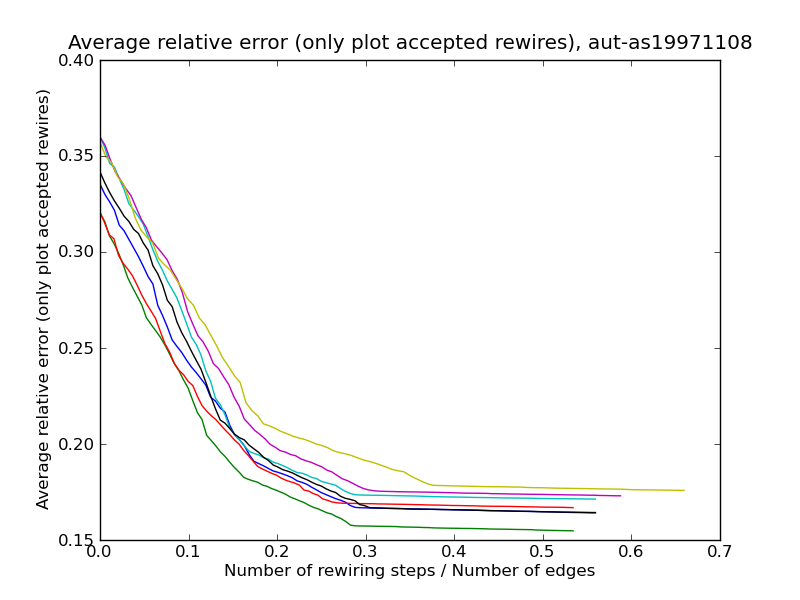
\includegraphics[scale=0.75]{acceptedOnly-aut-as19971108.png}\\
\end{figure}


\begin{figure}[p]
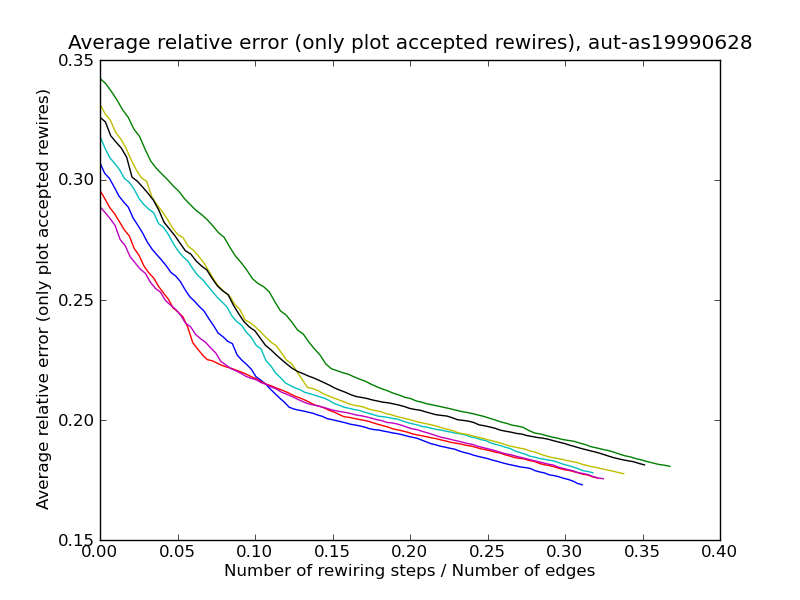
\includegraphics[scale=0.75]{acceptedOnly-aut-as19990628.png}\\
\end{figure}


\begin{figure}[p]
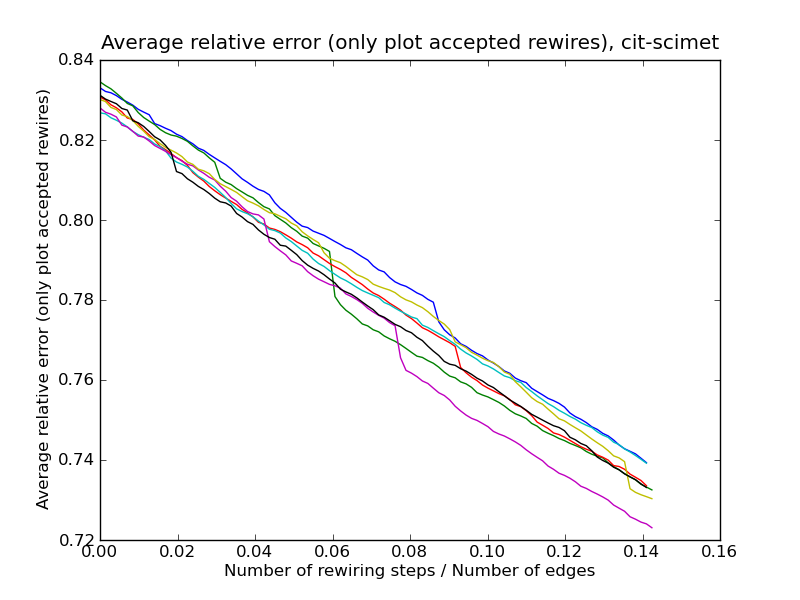
\includegraphics[scale=0.75]{acceptedOnly-cit-scimet.png}\\
\end{figure}


\begin{figure}[p]
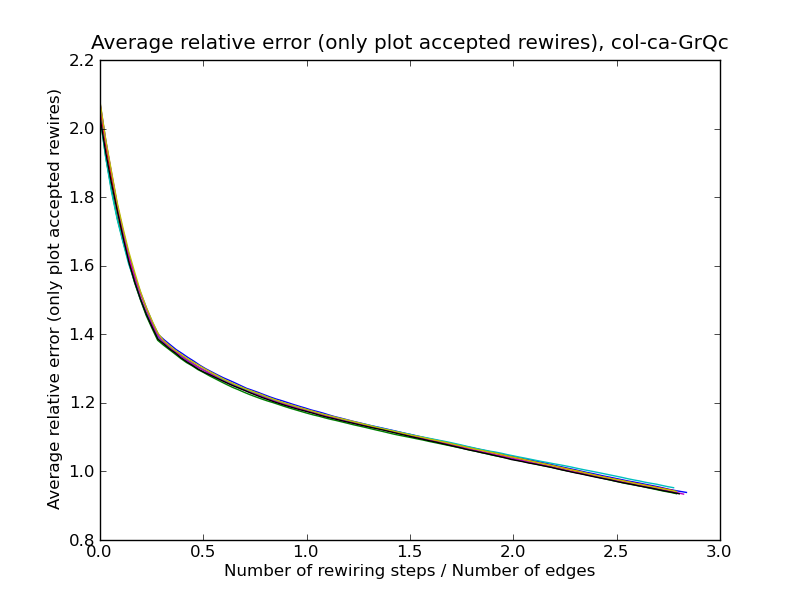
\includegraphics[scale=0.75]{acceptedOnly-col-ca-GrQc.png}\\
\end{figure}


\begin{figure}[p]
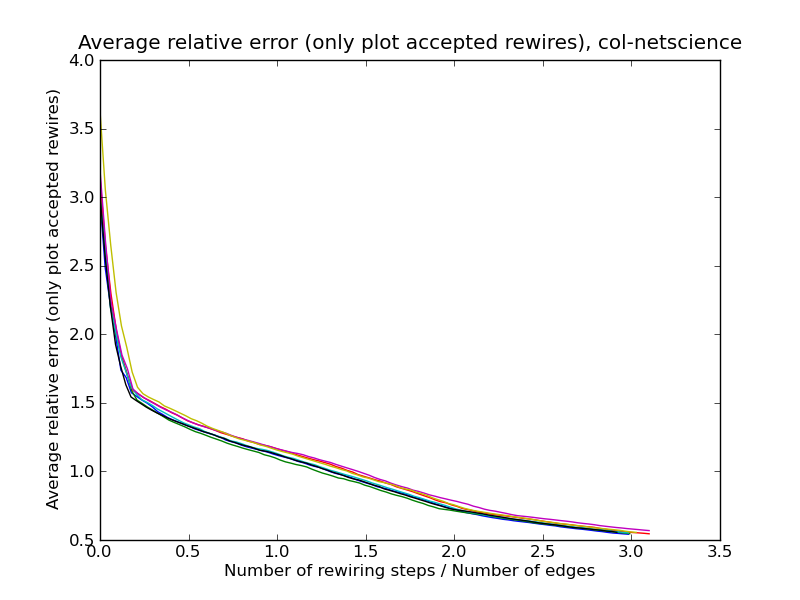
\includegraphics[scale=0.75]{acceptedOnly-col-netscience.png}\\
\end{figure}


\begin{figure}[p]
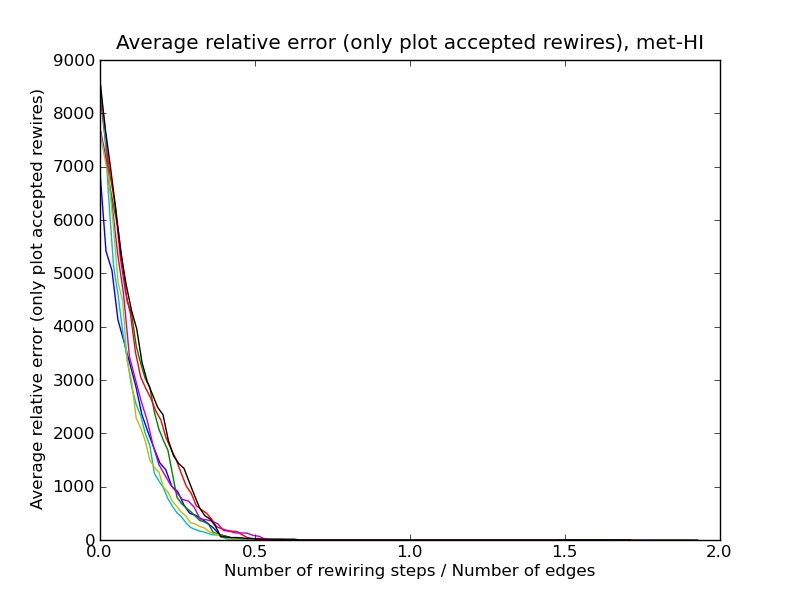
\includegraphics[scale=0.75]{acceptedOnly-met-HI.png}\\
\end{figure}


\begin{figure}[p]
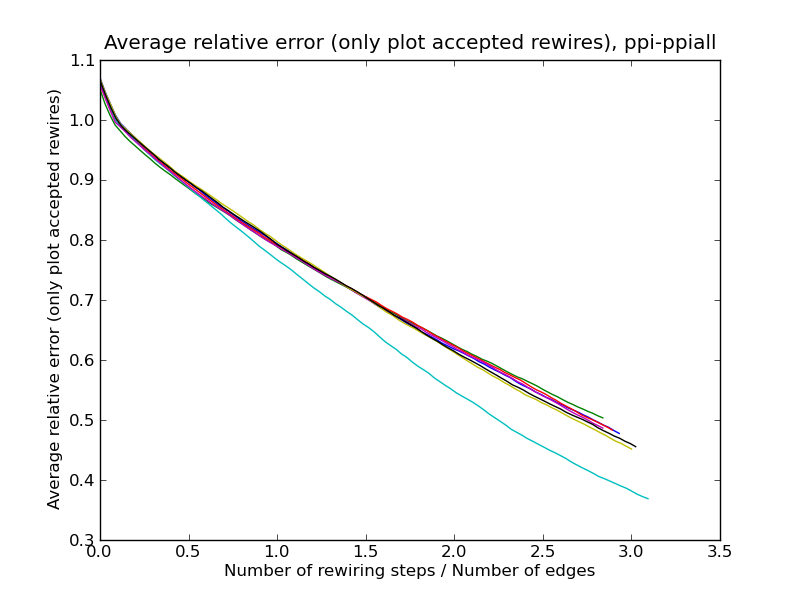
\includegraphics[scale=0.75]{acceptedOnly-ppi-ppiall.png}\\
\end{figure}


\begin{figure}[p]
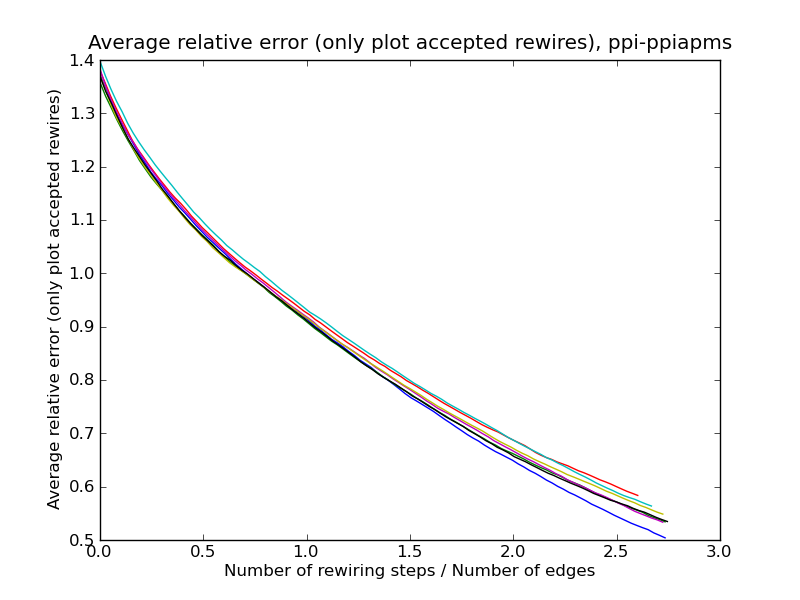
\includegraphics[scale=0.75]{acceptedOnly-ppi-ppiapms.png}\\
\end{figure}


\begin{figure}[p]
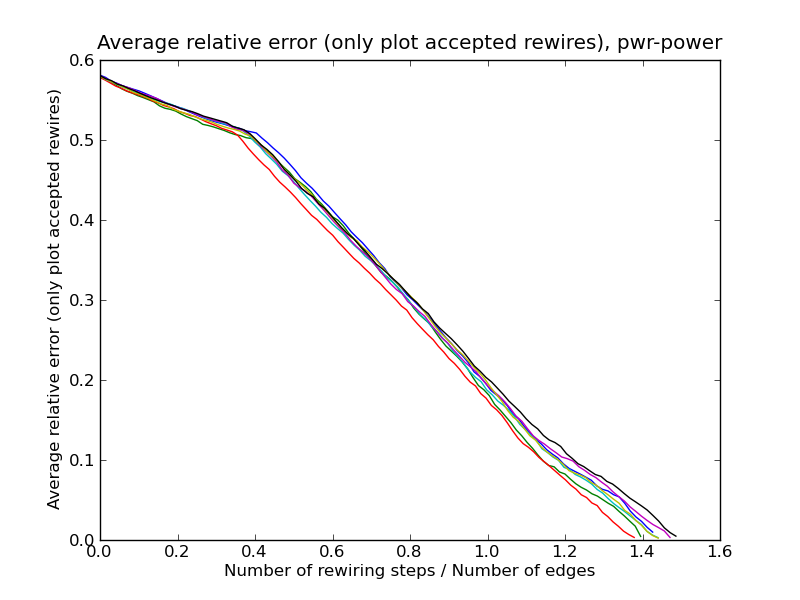
\includegraphics[scale=0.75]{acceptedOnly-pwr-power.png}\\
\end{figure}


\begin{figure}[p]
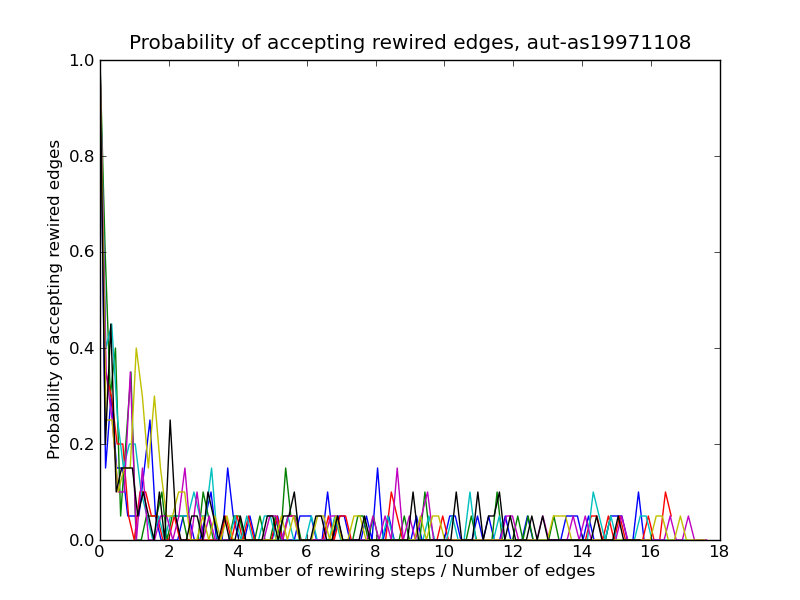
\includegraphics[scale=0.75]{Paccept-aut-as19971108.png}\\
\end{figure}

\begin{figure}[p]
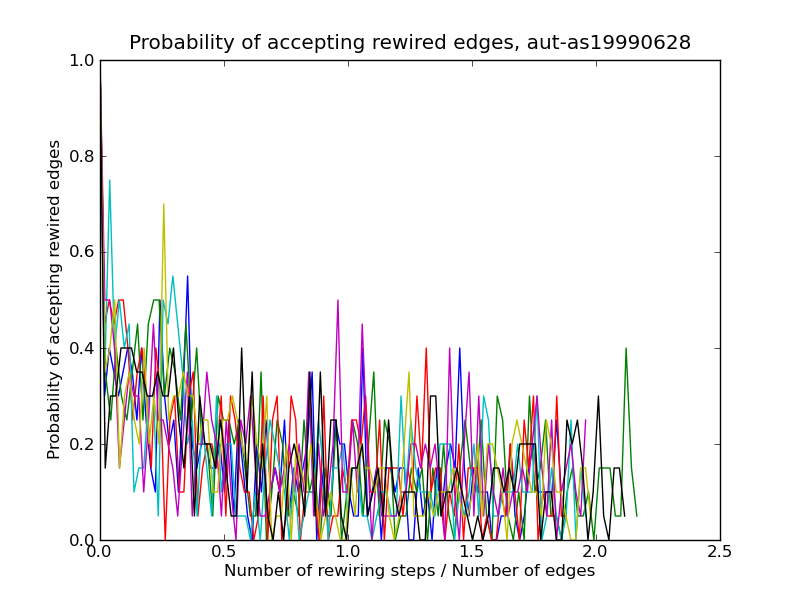
\includegraphics[scale=0.75]{Paccept-aut-as19990628.png}\\
\end{figure}

\begin{figure}[p]
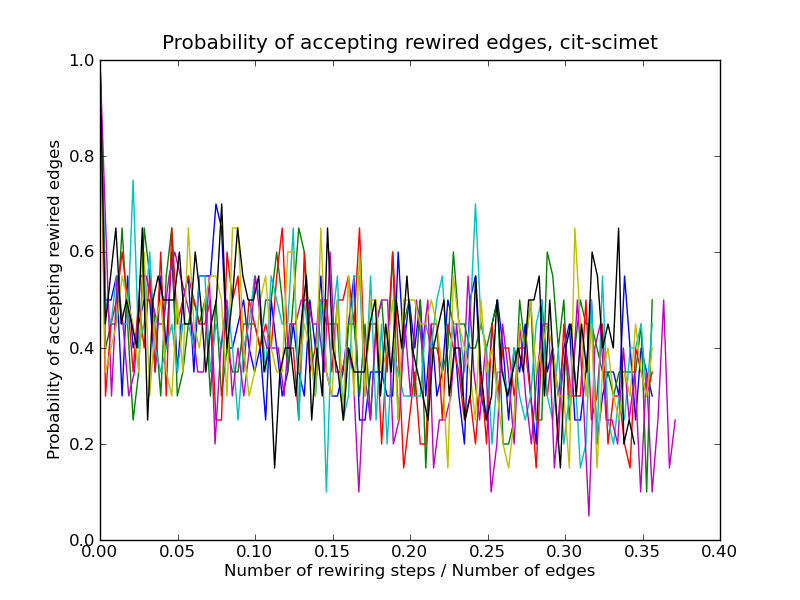
\includegraphics[scale=0.75]{Paccept-cit-scimet.png}\\
\end{figure}


\begin{figure}[p]
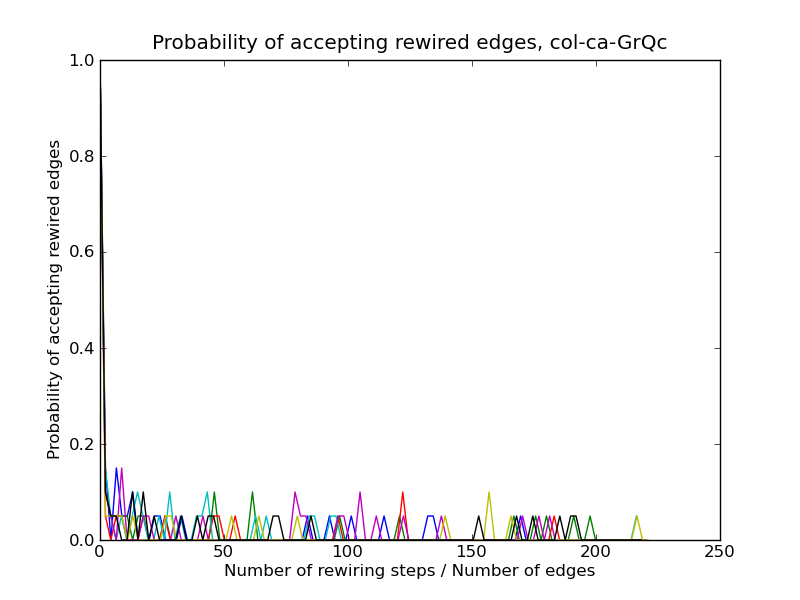
\includegraphics[scale=0.75]{Paccept-col-ca-GrQc.png}\\
\end{figure}


\begin{figure}[p]
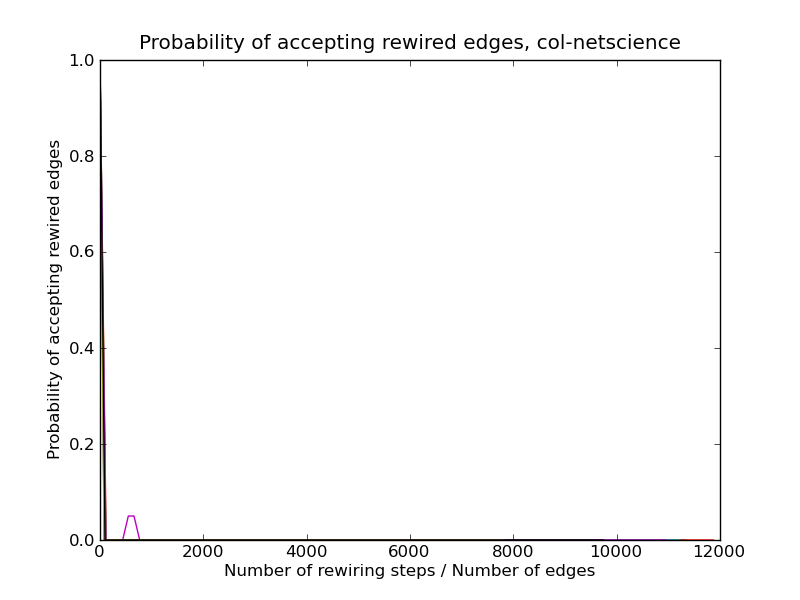
\includegraphics[scale=0.75]{Paccept-col-netscience.png}\\
\end{figure}


\begin{figure}[p]
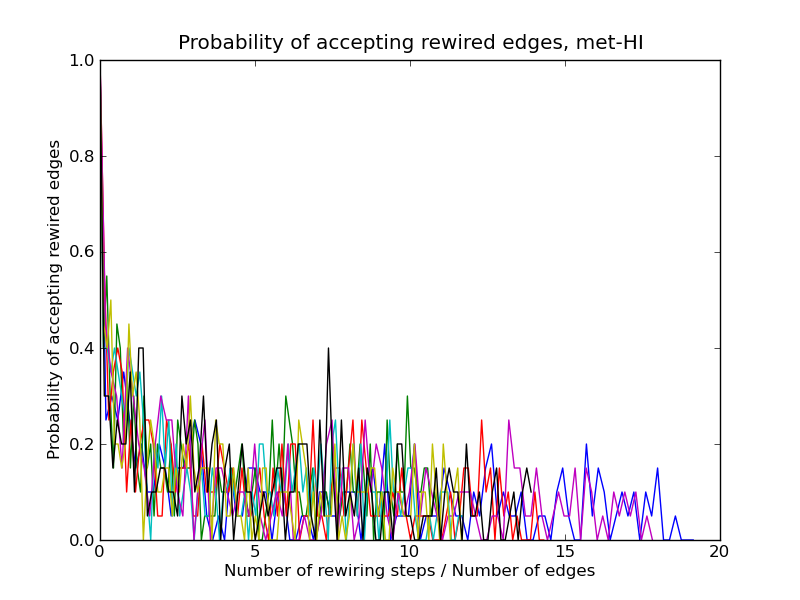
\includegraphics[scale=0.75]{Paccept-met-HI.png}\\
\end{figure}


\begin{figure}[p]
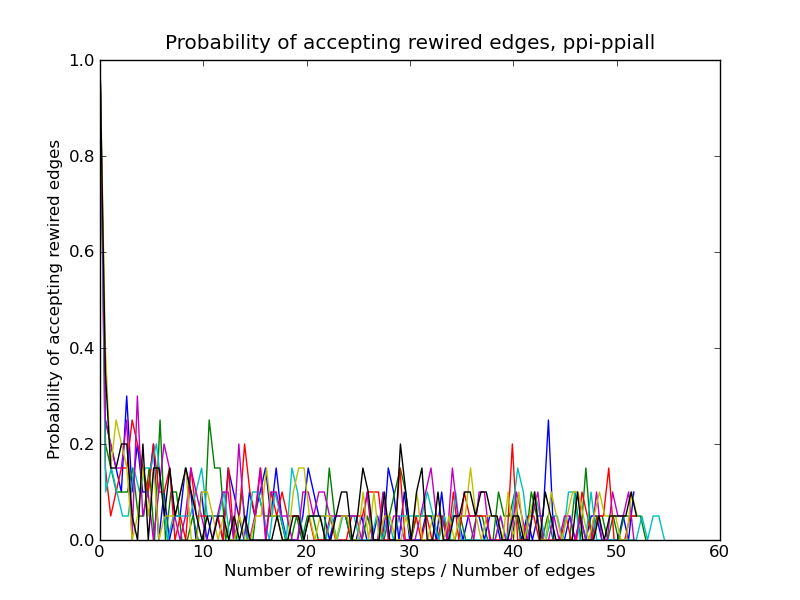
\includegraphics[scale=0.75]{Paccept-ppi-ppiall.png}\\
\end{figure}


\begin{figure}[p]
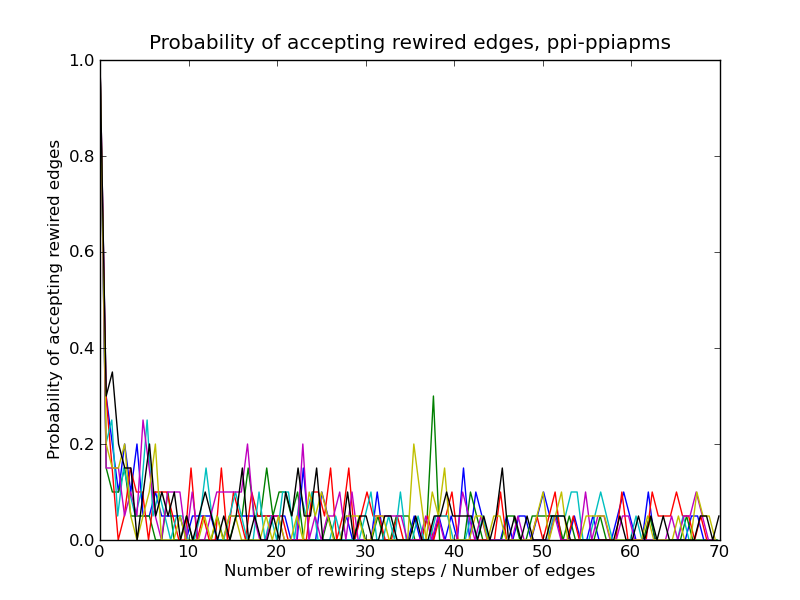
\includegraphics[scale=0.75]{Paccept-ppi-ppiapms.png}\\
\end{figure}


\begin{figure}[p]
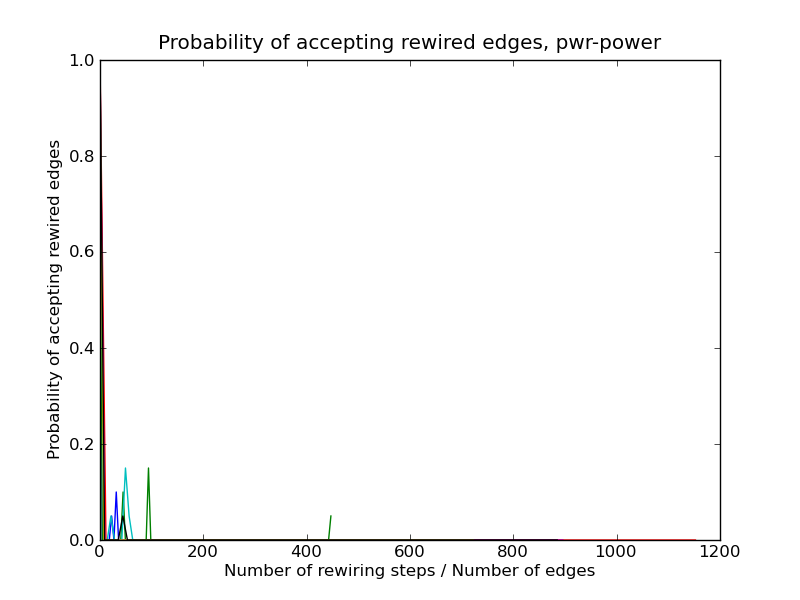
\includegraphics[scale=0.75]{Paccept-pwr-power.png}\\
\end{figure}




\end{document}